\section{Generative models}
In unsupervised learning we want to find generative models which allow us to generate new data
from previously made observations. We sometimes assume that observations are generated from a 
process which is not immediately observable from the data at hand. A general form of such a 
generative model can be written as:
\begin{align}
	\mb{x} = f(\mb{s})
	\label{eq:GM}
\end{align}
where $\mb{x}$ is a $D \times 1$ vector for a given observation, which is assumed to be 
generated by an arbitrary function $f(\mb{s})$. $\mb{s}$ is a $M \times 1$ vector of
source signals for the given observation. If $\mb{s}$ is known the problem of inferring
function $f(\mb{s})$ becomes a supervised learning task. However, if the sources are 
unknown the problem becomes an unsupervised learning task. UNder certain assumptions
it possible to infer sources from observations, this is called blind source separation.

\subsection{The linear generative model (LGM)} 
In the following we will only consider linear generative models for which equation \eqref{eq:GM}
takes the form:
\begin{align}
	\mb{x} = \mb{A s}
	\label{eq:LGM}
\end{align}
where $\mb{x}$ is an $D \times 1$ observation vector, $\mb{s}$ is the $M \times 1$ vector
of sources and $\mb{A}$ is a $D \times M$ transformation matrix. 
We distinguish three classes of LGM dependent on the dimensionality of $\mb{A}$:

\begin{enumerate}
	\item Overcomplete LGM: \textbf{A} is a fat matrix with $D<M$. \\
		  The number of source signals is assumed to be bigger than the dimensionality 
		  of our observations. The generative model is overcomplete since blow up the number
		  of possible sources.
	\item Undercomplete LGM: \textbf{A} is a flat matrix with $D>M$. \\
	      The undercomplete case is the inverse case an overcomplete LGM where the observations
	      are assumed to be generated from less sources that the dimensionality of our observations.
	\item Complete LGM: \textbf{A} is a square matrix with $D=M$, full rank 
	      and $\forall m = 1,\dots,M: \, \mathrm{Var}[\mb{s_m}] > 0.$ \\
	      In the complete case the number of source signals is assumed to equal the dimensionality
	      of our observations. In the following we will focus on complete LGMs.    
\end{enumerate}

% Table of UL algorithms used for different types of LGM
\begin{figure}[h]
\centering
\begin{tabular}{|l|l|}
\hline 
Generative Model & Unsupervised Learning algorithm \\ 
\hline 
Complete LGM & Principle Component Analysis (PCA), \\ 
             & Independent Components Analysis (ICA) \\ 
%\hline 
Overcomplete LGM & Factor Analysis, Independent Factor Analysis \\ 
\hline 
\end{tabular} 
\caption{Some examples of unsupervised leanring algorithms for the different classes of LGM. 
For all those algorithms it is assumed that observations \textbf{X} can be decomposed into 
sources $\mb{S}$ and transformation matrix $\mb{A}$.}
\end{figure}

\subsection{The complete LGM}
In this section we assume that our observations and signals have the same dimensionality,
i.e. we are dealing with a complete LGM. We further assume that matrix $\mb{A}$ is orthogonal
which means that:
\begin{align}
	 \mb{A}\TT \mb{A} = \mb{A} \mb{A}\TT = \imat_D
\end{align}
\noindent
We will further focus on normally distributed source signals as this will be relevant for the
orthogonality assumption with the application of principle component analysis. In fact orthogonality
of $\mb{A}$ is only guaranteed if our observations are normally distributed. We can show that given
the sources are normally distributed, our observations will be too:


%% From lecture
%\textbf{Linear mappings of Gaussian RVs:} \\
%$s \sim \	{N}(\mathbf{\mu_s},\mathbf{C_s})$
%\begin{align*}
%	x_k &= a_k s_1 + b_k s_2 \\
%	s_j &\sim \mathcal{N}(0,\sigma_j^2); \qquad \rho(s_1,s_2) = \rho(s_1)\rho(s_2) \\
%	\Rightarrow x_n &\sim \mathcal{N}(0,a_k^2 \sigma_1^2 + b_k^2 \sigma_2^2)
%\end{align*}

\begin{proposition}[Linear mappings of Gaussian random variables]
Given the sources are independent and normally distributed such that
\begin{align*}
	\mb{s} \sim \mathcal{N}(\greekvec{\mu}_s,\mb{C_s}); \qquad
	\rho(\mb{s}) = \prod_{m=1}^M \rho(s_m); \qquad
	s_m \sim \mathcal{N}(0,\sigma_m^2) &
\end{align*}
and the observations are linear mappings of the sources such that
\begin{align*}
	x_d = \sum_{m=1}^M \mb{A}_{dm} s_m
\end{align*}
The observations will be normally distributed according to
\begin{align*}
	x_d \sim \mathcal{N}(0, \sum_{m=1}^M \mb{A}_{dm}^2 \sigma_m^2)
\end{align*}
\end{proposition}

\begin{proof}[Sketch of proof.]
	\begin{align*}
	(i) &\qquad (\mb{A}_{dm} s_m) \sim \mathcal{N}(0,\mb{A}_{dm}^2 \sigma_m^2) \\
	(ii) &\qquad \text{generally for } \\
		 &\qquad z = u + v : \rho(z) = \underbrace{\rho(u) \Asterisk \rho(v)}_{\text{Convolution}}\\
	     &\qquad \Rightarrow \underbrace{\mathcal{F}[\rho(z)]}_{\text{Fourier transform}} 
	       = \underbrace{\underbrace{\mathcal{F}[\rho(u)]}_{Gaussian} \underbrace{\mathcal{F}[\rho(v)]}_{Gaussian} }_{Gaussian} \\
	     &\qquad \Rightarrow \rho(z) = \underbrace{\mathcal{F}^{-1}(\cdots)}_{Gaussian}
\end{align*}
\end{proof}
\noindent 
The density of the sum of two random variables is obtained by convolving their individual densities. 
The convolution of two Gaussians is a multiplication of two Gaussians in the Fourier space. Backtransformation again results
in a Gaussian. Below we will see how the covariance $\mb{C}_x$ of observations $\mb{x}$ can be decomposed given an LGM.

%Sketch of proof:
%\begin{align*}
%	(i) &\qquad (a_k s_1) \sim \mathcal{N}(0,a_k^2 \sigma_1^2) \\
%	    &\qquad (b_k s_2) \sim \mathcal{N}(0,b_k^2 \sigma_2^2)	\\
%	(ii) &\qquad \text{generally for } \\
%		 &\qquad z = u + v : f(z) = f(u) + f(v)\\
%	     &\qquad \Rightarrow \underbrace{\mathcal{F}[f(z)]}_{\text{Fourier transform}} 
%	       = \underbrace{\underbrace{\mathcal{F}[f(u)]}_{Gaussian} \underbrace{\mathcal{F}[f(v)]}_{Gaussian} }_{Gaussian} \\
%	     &\qquad \Rightarrow f(z) = \underbrace{\mathcal{F}^{-1}(\cdots)}_{Gaussian}
%\end{align*}
%Aside: The Fourier transform of a density $\hat{=}$ the characteristic function $\E_{\rho(z)}[\E^{ikz}]$

\begin{theorem}[Linear transform theorem]
Given $\mb{x} = \mb{A s}$ is a linear mapping and $\mb{s}$ and $\mb{x}$ are normally distributed such that
\begin{align*}
	\mb{s} \sim \mathcal{N}(\greekvec{\mu}_s,\mb{C}_s) \qquad
	\text{ and } \qquad
	\mb{x} \sim \mathcal{N}(\greekvec{\mu}_x,\mb{C}_x) \qquad
\end{align*}
then the expectation and covariance of $\mb{x}$ are given by
\begin{align*}
	(i)& \qquad \greekvec{\mu}_x = \mb{A} \greekvec{\mu}_s \\
	(ii)&  \qquad \mathbf{C}_x = \mathbf{A} \mathbf{C}_s \mathbf{A}\TT %
\end{align*}
where we refer to $(ii)$ as the "Sandwich theorem".
\end{theorem}

\begin{proof}[Derivation]
\qquad \\
\begin{minipage}{0.45\textwidth}
\begin{align*}
	\greekvec{\mu}_x &= \Ex{\rho(\mb{x})}{\mb{x}} \\
	                 &= \Ex{\rho(\mb{x})}{\mb{A s}} \\
	                 &= \mb{A} \Ex{\rho(\mb{s})}{\mb{s}} \\
	                 &= \mathbf{A} \greekvec{\mu}_s \\
\end{align*}
\end{minipage}
\begin{minipage}{0.45\textwidth}
\begin{align*}
	\mb{C}_x &= \Ex{}{\mb{x x}\TT} - \Ex{}{\mb{x}} \Ex{}{\mb{x}}\TT \\
		     &= \Ex{}{\mathbf{A s s }\TT \mb{A}\TT} 
				    - \Ex{}{\mb{A s}} \Ex{}{\mb{s}\TT \mathbf{A}\TT} \\
				 &= \mb{A} \Ex{}{\mathbf{s s}\TT} \mb{A}\TT 
				    - \mb{A} \Ex{}{\mathbf{s}} \Ex{}{\mb{s}}\TT \mb{A}\TT \\
				 &= \mathbf{A} \left(\Ex{}{\mathbf{s s}\TT} - \Ex{}{\mathbf{s}} \Ex{}{\mb{s}}\TT \right) \mathbf{A}\TT \\
				 &= \mathbf{A} \mathbf{C}_s \mathbf{A}\TT \\
\end{align*}
\end{minipage}
\newline
\end{proof}

%\begin{align*}
%	\mathbf{u} &= \mathbf{W v} \\
%	\rho(\mathbf{v}) &= \mathcal{N}(\mathbf{v}|\greekvec{\mu_v},\mathbf{C_v})\\
%	\rho(\mathbf{u}) &= \mathcal{N}(\mathbf{u}|\greekvec{\mu_u},\mathbf{C_u})\\
%	\greekvec{\mu_u} &= \Ex{\rho(\mathbf{u})}{\mathbf{u}}
%	                  = \Ex{\rho(\mathbf{u})}{\mathbf{W v}}
%	                  = \mathbf{W} \E_{f(\mathbf{u})}[\mathbf{v}] = \mathbf{W} \greekvec{\mu_v} \\
%	\mathbf{C_u} &= \E[\mathbf{u u}\TT] - \E[\mathbf{u}] \E[\mathbf{u}]\TT \\
%				 &= \E[\mathbf{W v v}\TT \mathbf{W}\TT] 
%				    - \E[\mathbf{W v}] \E[\mathbf{v}\TT\mathbf{W}\TT] \\
%				 &= \mathbf{W} \E[\mathbf{v v}\TT] \mathbf{W}\TT 
%				    - \mathbf{W} \E[\mathbf{v}] \E[\mathbf{v}]\TT \mathbf{W}\TT \\
%\end{align*}

%\begin{proposition}[Rules for expectations of linear mappings]
%	\begin{align*}
%		(i)& \qquad \Ex{}{\mathbf{W v}} = \mathbf{W} \Ex{}{\mathbf{v}} \\
%		(ii)&  \qquad \Ex{}{\mathbf{A X B}} = \mathbf{A} \Ex{}{\mathbf{X}} \mathbf{B} %
%	\end{align*}		
%\end{proposition}
%
%\begin{theorem}[Linear transform theorem]
%	\begin{align*}
%		\mathbf{u}  = \mathbf{W v}
%	\end{align*}
%
%	\begin{align*}
%		(i)& \qquad \greekvec{\mu_u} = \mathbf{W} \greekvec{\mu_v} \\
%		(ii)&  \qquad \mathbf{C_u} = \mathbf{W} \mathbf{C_v} \mathbf{W}\TT %
%	\end{align*}		
%	We call this the "Sandwich theorem"
%\end{theorem}

\noindent We can now apply the sandwich theorem to calculate the covariance of a normally distributed random
variable with independent normally distributed sources as sketched above.
\begin{proposition}[Covariance matrix for observations from independent normally distributed sources]
Given
	\begin{align*}
		\mb{s} \sim \mathcal{N}(\greekvec{\mu}_s,\mb{C_s}); \qquad
		\rho(\mb{s}) = \prod_{m=1}^M \rho(s_m); \qquad
		\mb{C}_s = \mathrm{diag}(\sigma_1^2, \dots ,\sigma_M^2) &
	\end{align*}
then
	\begin{align}
		\begin{split}
		\mathbf{C}_x &= \mb{A} \mb{C}_s \mb{A}\TT \\
		             &= \sum_{m=1}^M \sigma_m^2 \underbrace{\mathbf{a_m a_m\TT}}_{\text{rank-1-matrix outer product}}
		             \label{eq:Cx}
		\end{split}
	\end{align}
where $\mathbf{a_m}$ is a $D \times 1$ basis vector of matrix $\mb{A}$.
\end{proposition}

\noindent For visualization of the source covariance before transformation and the covariance of the observations
after applying $\mb{A}$ to the sources we introduce another transformation which yields a one-dimensional 
marginal distribution.

\begin{proposition}[Variance contour lines]
Take an arbitrary $D \times 1$ vector $\mb{w}$ with $\|\mathbf{w}\| = 1$ such that
	\begin{align}
		&u = \mathbf{w\TT x}
	\end{align}
\noindent yields a one-dimensional marginal distribution. For a covariance of $\mb{x}$ as shown in equation
\eqref{eq:Cx} the variance of $u$ is given by
\begin{align}
\begin{split}
	\mathrm{Var}[u] &= \mathbf{w C_x w} \\
	                          &= \mathbf{w}\TT \left(\sum_{m=1}^M \sigma_m^2 \mathbf{a_m a_m\TT}\right) \mathbf{w} \\
	                          &= \sum_{m=1}^M \sigma_m^2 (\mathbf{w\TT a_m}) (\mathbf{a_m\TT w}) \\
	                          &= \sum_{m=1}^M \sigma_m^2 (\mathbf{w\TT a_m})^2 \label{eq:Cu}
\end{split}
\end{align}
We notice that the marginalization introduces a projection of the basis vectors of $\mb{A}$ onto the axis that is
spanned by $\mb{w}$ where the variance $\mathrm{Var}[u]$ is the variance along $\mb{w}$. We can now calculate 
the variance along any direction in the sample space and visualize it using variance contour lines.
\end{proposition}

\subsubsection{Example for three LGM with different source distributions}
To inspect the influence of the linear transformation on the covariance of the sources we utilize the above 
marginalization to calculate variance contour lines. We will distinguish three cases of source distributions,
two of which are Gaussians and one is a uniform distribution. For visualization purposes we will focus on 2-dimensional
examples although the approach can be applied to cases with higher dimensions.

\paragraph{Special case: Isovariance with $\sigma_1^2 = \dots = \sigma_M^2 = \sigma^2$}
\label{par:cov_isovar}
\qquad \newline
Given
	\begin{align*}
		\mb{s} \sim \mathcal{N}(\greekvec{\mu}_s,\mb{C_s}); \qquad
		\mathbf{C_s} &= \sigma^2 \imat_M &
	\end{align*}
	
\begin{minipage}{0.45\textwidth}
\begin{align*}
	\mathbf{C_x} &= \mathbf{A C_s A\TT} \\
	             &= \sigma^2 \mathbf{A} \imat_M \mathbf{A}\TT \\
	             &= \sigma^2 \underbrace{\mathbf{A}\mathbf{A}\TT}_{\mathbf{A}\text{ is orthogonal}} \\
	             &= \sigma^2 \imat_M = \mathbf{C_s} \\
\end{align*}
\end{minipage}
\begin{minipage}{0.45\textwidth}
\begin{align*}
	\mathrm{Var}[\mb{w\TT x}] &= \mathbf{w\TT C_x w} \\
				    &= \mathbf{w\TT C_s w} \\
	                &= \sigma^2 \mathbf{w}\TT \imat_M \mathbf{w} \\
	                &= \sigma^2 \mathbf{w}\TT \mathbf{w} \\
	                &= \sigma^2 \|\mathbf{w}\|^2 = \sigma^2 \\
\end{align*}
\end{minipage}
\newline
We see that given the source distribution has isovariance and the transformation matrix $\mb{A}$ is orthogonal
the corvariance of observations will have the same covariance as the source distribution. In turn the variance
of the introduced marginalization will be constant for any $\mb{w}$ with $\|\mathbf{w}\|^2 = 1$. 
\figref{fig:LGM_isovar} illustrates the variance contour lines for the three cases.
With the next two cases we will focus on visual inspection of the contour lines without making any further
derivations.

\begin{figure}
	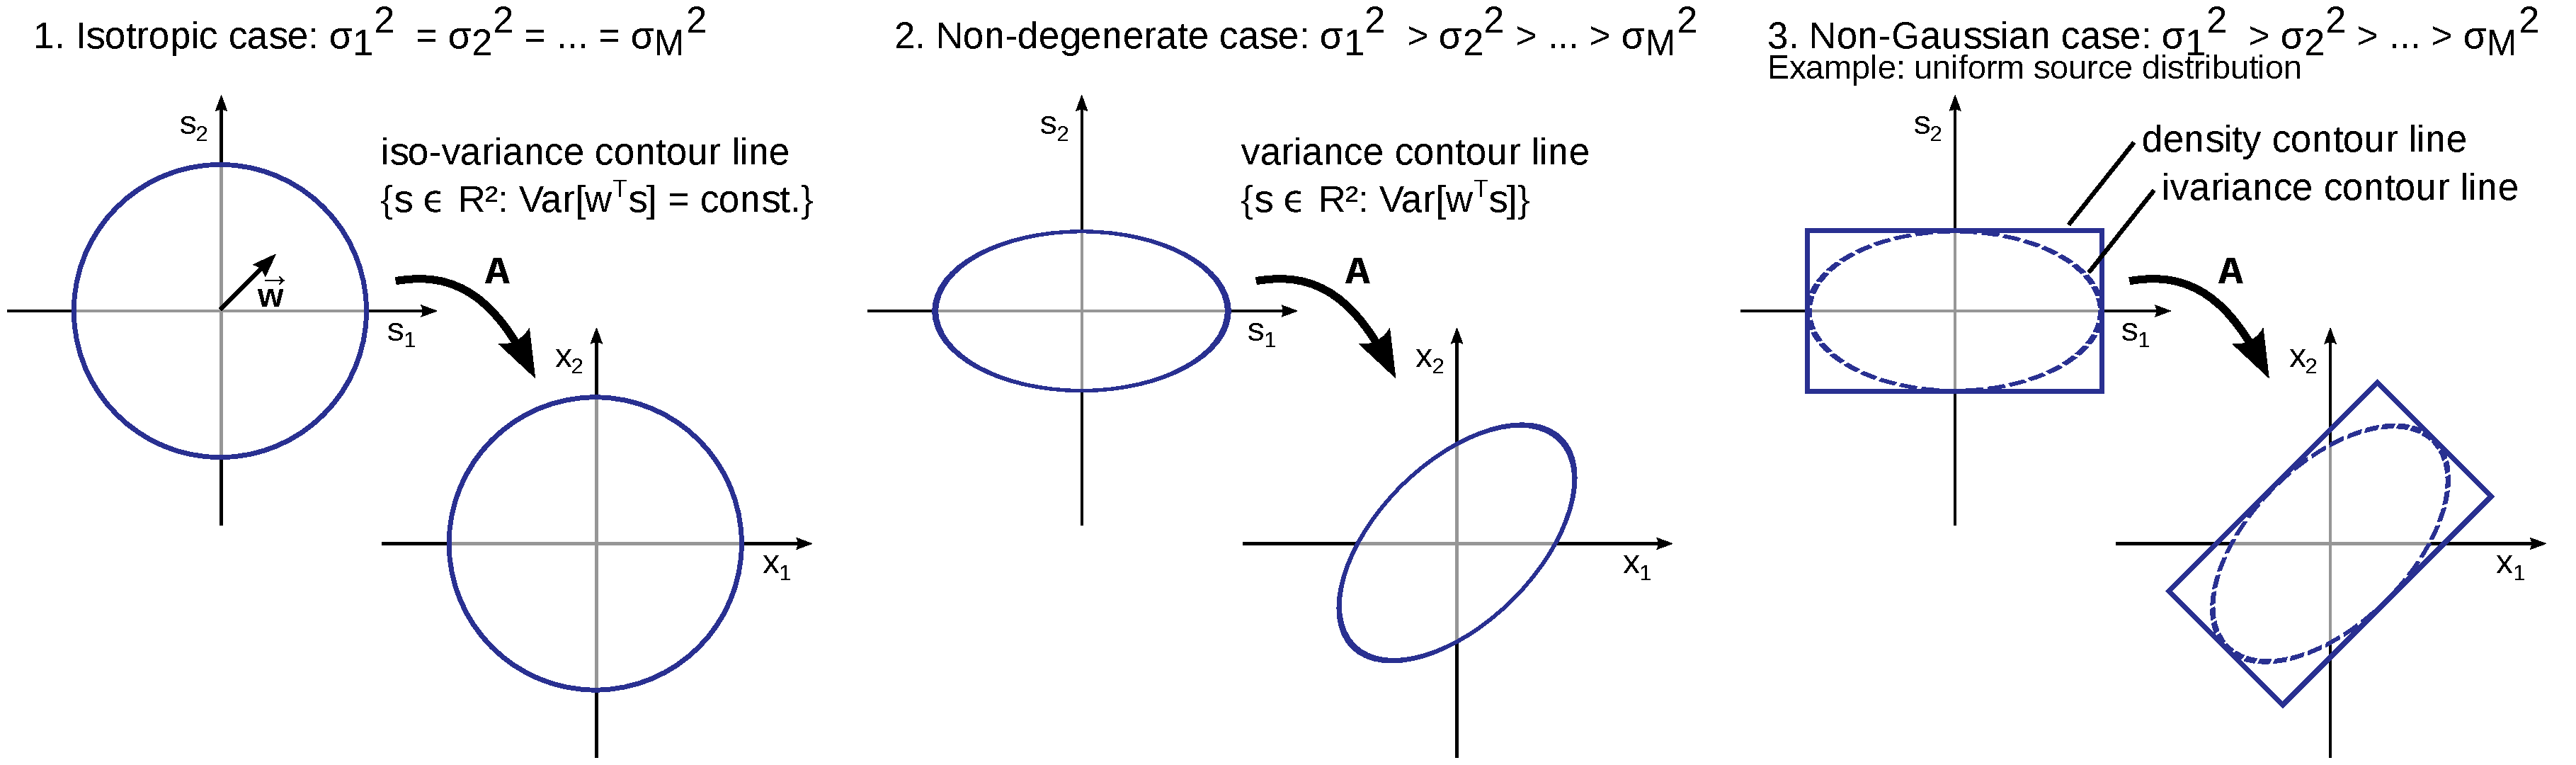
\includegraphics[width=\textwidth]{./lecture10/lineartransform_geometricmeaning.pdf}
	\caption{Variance contour lines before and after applying $\mb{A}$.}
	\label{fig:LGM_isovar}
\end{figure}

\paragraph{Non-degenerate case: $\sigma_1^2 > \sigma_1^2 > \dots > \sigma_M^2$}
Given the source distribution is a Gaussian with independent sources and unequal source variances.
We see that applying matrix $\mb{A}$ can introduce a rotation of the variance contour line and in turn
introduces correlation for the dimensions of $\mb{x}$. That is, although the source were perfectly 
independent the matrix $\mb{A}$ introduces correlations. It becomes apparent that if we find a matrix
$\mb{A}^{-1}$ which can be applied to the data, we can remove those correlations.

\paragraph{Non-Gaussian case: $\sigma_1^2 > \sigma_1^2 > \dots > \sigma_M^2$}
In this case we assume a uniform source distribution with unequal source variances. Although the
density contour line differs from the variance contour line under the Gaussian assumption we see
that applying $\mb{A}$ introduces the same correlations in the observations as in the Gaussian
case.

\subsection{Blind source separation}
If we make observations which are correlated and we assume that the sources are uncorrelated we
can find a tranform $\mb{A}\TT$ which removes correlations and recovers the uncorrelated signals.
We call this approach whitening. But how can we uniquely identify $\mb{A}$?

\begin{proposition}[Sufficient condition]
	If we assume that $\sigma_1^2 > \sigma_2^2 > \dots > \sigma_k^2$ and if we assume an orthogonal LGM
	then we can uniquely identify $\mathbf{A}$ and the solution is given by the Eigenvectors of the convariance
	matrix $\mathbf{C_x}$ of the data. This is what we call principle component analysis.
\end{proposition}